\documentclass[11pt,a4paper]{article}
\usepackage[margin=2.2cm]{geometry}
\usepackage{amsmath,amssymb}
\usepackage{booktabs}
\usepackage{graphicx}
\usepackage[hidelinks]{hyperref}
\usepackage{caption}
\captionsetup{font=small,labelfont=bf}
\usepackage{microtype}
\setlength{\parskip}{3pt}

\title{Volatility is rough: replication and forecasting\\[2pt]
\large A 31-index replication of Gatheral, Jaisson \& Rosenbaum (2018)\\ and an out-of-sample forecasting competition}
\author{Polina Ptukha\\ M2 MASEF, Universit\'e Paris Dauphine--PSL}
\date{October 2026}

\begin{document}
\maketitle

\begin{abstract}
\noindent
Using 5-minute realized variance for 31 equity indices (Oxford-Man Realized Library, 2000--2022) we
re-estimate the roughness of log-volatility. The scaling $m(q,\Delta)\propto\Delta^{qH}$ holds well,
and the median Hurst exponent is $H=0.126$ (range 0.079--0.171; S\&P 500: $0.149\pm0.021$), in line with the
paper. Range-based (Garman--Klass) variance from daily OHLC, extended to October 2026 for 20 indices,
gives a lower median $H=0.077$, consistent with measurement noise pulling $H$ down. In a walk-forward
competition (validation up to 2014, untouched test period from 2015), the paper's RFSV predictor is
\emph{not} better than HAR at 1 day (worse on 17 of 31 indices by Diebold--Mariano at 5\%), is level with HAR at
5 days and marginally better on average at 20 days (not significant on any index). A HAR model with a
leverage term and the RFSV forecast as an extra regressor, chosen on the validation period, lowers the
test log-MSE relative to HAR by 5.9\% (1 day) and, with a forecast combination, by 1.8\% (5 days) on the RV data; it
beats both HAR and RFSV on every index at 1 day. At 20 days the validation-chosen model (rolling-$H$ RFSV)
does not beat either benchmark on the test period.
\end{abstract}

\section{Introduction}
Gatheral, Jaisson and Rosenbaum (GJR, 2018) showed that the log of realized volatility behaves like
a fractional Brownian motion (fBm) with Hurst exponent $H\approx 0.1$, far below the $H>1/2$ of the
long-memory models used before. Two consequences follow: volatility paths are \emph{rough}, and the
conditional expectation of future log-volatility has a closed form, which the authors use as a
forecasting rule (the RFSV predictor) and find to be competitive with the HAR model of Corsi (2009).
This project (i) replicates the estimation on all 31 indices of the Oxford-Man library and on a
range-based series to 2026, (ii) checks two side claims (Gaussian increments and the smoothing bias),
and (iii) runs a walk-forward forecasting competition with an honest validation/test split, including
attempts to improve on both RFSV and HAR.

\section{Data}
\textbf{Realized variance (RV).} 5-minute realized variance (\texttt{rv5}) and open-to-close returns
for 31 indices from the final public version of the Oxford-Man Institute Realized Library
(Heber, Lunde, Shephard \& Sheppard, 2009), 3 January 2000 -- 25 February 2022, obtained from the
Internet Archive copy of the official zip (snapshot of 1 March 2022). The library was discontinued in
2022 and has no open licence; it was free for academic research with citation, so the data are not
redistributed with the code.
\textbf{Range-based variance (GK).} Daily OHLC for 20 indices from Yahoo Finance (via \texttt{yfinance}),
January 2000 -- 12 October 2026. Daily variance is the Garman--Klass estimator
$\tfrac12(\log H/L)^2-(2\log2-1)(\log C/O)^2$; Parkinson's $(\log H/L)^2/(4\log2)$ is a cross-check
(correlation of logs 0.91--0.97). Days with zero range, prices outside $[L,H]$ or non-positive GK are
dropped (at most 11 days per index). The correlation between $\log$RV and $\log$GK on overlapping days is
0.77--0.91.
The two data types are \emph{never mixed} in one series; every result is reported separately for RV and GK.
Throughout, $\log\sigma_t=\tfrac12\log v_t$ with $v_t$ the daily variance proxy, and time is counted in
trading days of each index.

\section{Replication}
\subsection{Scaling of log-volatility increments}
For $q\in\{0.5,1,1.5,2,3\}$ and $\Delta=1,\dots,50$ we compute
$m(q,\Delta)=\frac{1}{N-\Delta}\sum_t|\log\sigma_{t+\Delta}-\log\sigma_t|^q$.
If $\log\sigma_t-\log\sigma_s\sim\nu\,|t-s|^H Z$ with $Z\sim N(0,1)$, then
$m(q,\Delta)=\nu^q\,\mathbb E|Z|^q\,\Delta^{qH}$, so an OLS regression of $\log m(q,\Delta)$ on $\log\Delta$
has slope $\zeta_q=qH$. We estimate $H$ as the slope of $\zeta_q$ on $q$ through the origin, and $\nu$ from
the $q=2$ intercept. Standard errors come from a block bootstrap: the series is cut into 250-day
blocks, the sums $\sum|\text{increment}|^q$ and pair counts are computed inside each block, and blocks are
resampled with replacement (500 draws). Figure~\ref{fig:scaling} shows the S\&P 500 case: the
$\log m$--$\log\Delta$ lines are straight and $\zeta_q$ is linear in $q$ (monofractal), as in the paper.

\begin{figure}[h]
\centering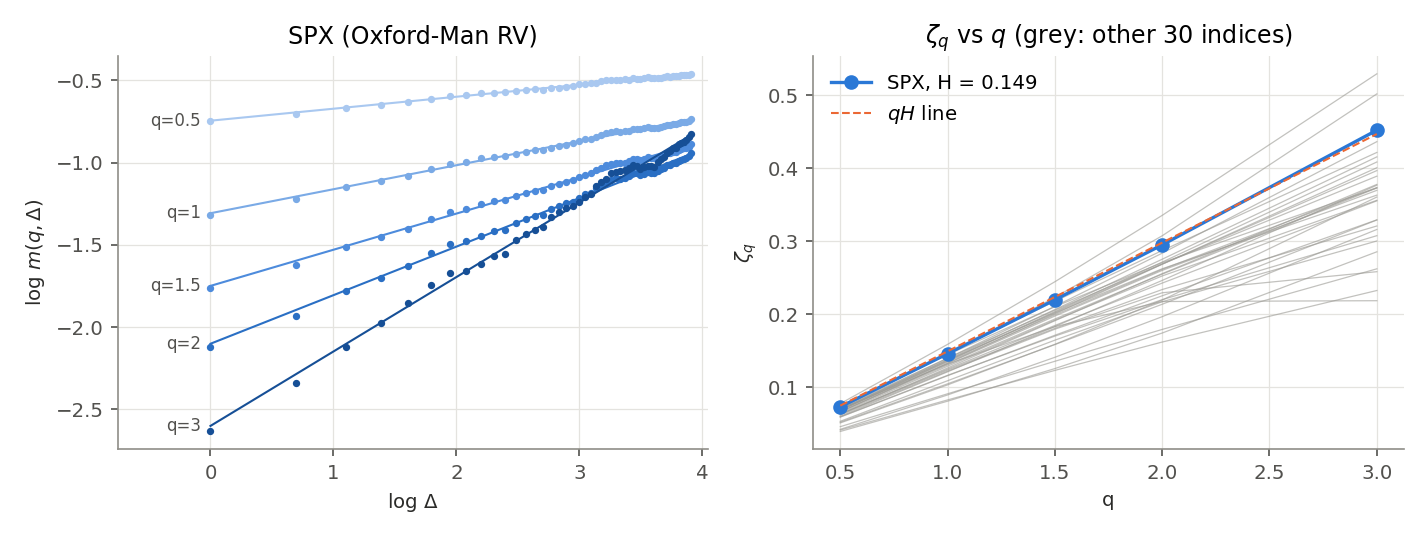
\includegraphics[width=0.92\textwidth]{../figures/scaling_spx.png}
\caption{Left: $\log m(q,\Delta)$ against $\log\Delta$ for the S\&P 500 (RV), with OLS fits.
Right: $\zeta_q$ against $q$; SPX in blue, the other 30 indices in grey.}
\label{fig:scaling}
\end{figure}

\begin{table}[h]
\centering\footnotesize
\resizebox{\textwidth}{!}{\begin{tabular}{lrrr@{\hskip 18pt}lrrr}
\toprule
Index & $H_{RV}$ (s.e.) & $H_{GK}$ (s.e.) & $\nu_{RV}$ & Index & $H_{RV}$ (s.e.) & $H_{GK}$ (s.e.) & $\nu_{RV}$\\
\midrule
AEX & 0.142 (0.019) & 0.072 (0.013) & 0.30 & KSE & 0.124 (0.017) & -- & 0.40\\
AORD & 0.090 (0.021) & 0.056 (0.015) & 0.37 & MXX & 0.079 (0.011) & 0.048 (0.008) & 0.38\\
BFX & 0.138 (0.017) & -- & 0.28 & N225 & 0.134 (0.019) & 0.075 (0.012) & 0.32\\
BSESN & 0.120 (0.010) & 0.078 (0.011) & 0.32 & NSEI & 0.107 (0.010) & 0.072 (0.016) & 0.35\\
BVLG & 0.160 (0.046) & -- & 0.24 & OMXC20 & 0.104 (0.013) & -- & 0.33\\
BVSP & 0.133 (0.016) & 0.067 (0.008) & 0.31 & OMXHPI & 0.112 (0.017) & -- & 0.33\\
DJI & 0.136 (0.020) & 0.092 (0.015) & 0.36 & OMXSPI & 0.127 (0.018) & -- & 0.32\\
FCHI & 0.133 (0.017) & 0.078 (0.011) & 0.30 & OSEAX & 0.108 (0.020) & -- & 0.35\\
FTMIB & 0.127 (0.022) & -- & 0.32 & RUT & 0.100 (0.022) & 0.072 (0.011) & 0.37\\
FTSE & 0.111 (0.014) & 0.075 (0.010) & 0.35 & SMSI & 0.128 (0.013) & -- & 0.31\\
GDAXI & 0.127 (0.018) & 0.079 (0.011) & 0.31 & SPX & 0.149 (0.021) & 0.094 (0.014) & 0.35\\
GSPTSE & 0.114 (0.026) & 0.079 (0.019) & 0.37 & SSEC & 0.131 (0.010) & -- & 0.33\\
HSI & 0.089 (0.013) & 0.054 (0.007) & 0.29 & SSMI & 0.171 (0.025) & 0.086 (0.014) & 0.25\\
IBEX & 0.126 (0.019) & 0.071 (0.012) & 0.29 & STI & 0.101 (0.029) & -- & 0.25\\
IXIC & 0.143 (0.019) & 0.083 (0.011) & 0.32 & STOXX50E & 0.093 (0.015) & 0.083 (0.009) & 0.38\\
KS11 & 0.123 (0.015) & 0.078 (0.009) & 0.28 & & & &\\
\midrule
\multicolumn{8}{l}{Median $H$: RV 0.126 (31 indices, range 0.079--0.171); GK 0.077 (20 indices, range 0.048--0.094).}\\
\bottomrule
\end{tabular}}
\caption{Estimated $H$ (block-bootstrap s.e.) from 5-minute RV (2000--2022) and from Garman--Klass
variance (2000--2026), and the vol-of-log-vol $\nu$ (RV, daily units).}
\label{tab:h}
\end{table}

Table~\ref{tab:h} reports every index. With RV, 25 of 31 estimates lie in $[0.10,0.15]$ (4 below, 2 above), the median is
0.126 and none exceeds 0.18: the paper's finding is confirmed across markets. The bootstrap standard errors
(typically 0.015--0.02) are larger than a naive i.i.d.\ calculation would give, because $H$ moves between
calm and stressed years. For a few indices (STOXX50E, RUT) $\zeta_q/q$ falls with $q$, i.e.\ the
largest moves scale less steeply; for most it is flat. The GK estimates are systematically lower
(median 0.077), and Figure~\ref{fig:h} shows this holds index by index.

\begin{figure}[h]
\centering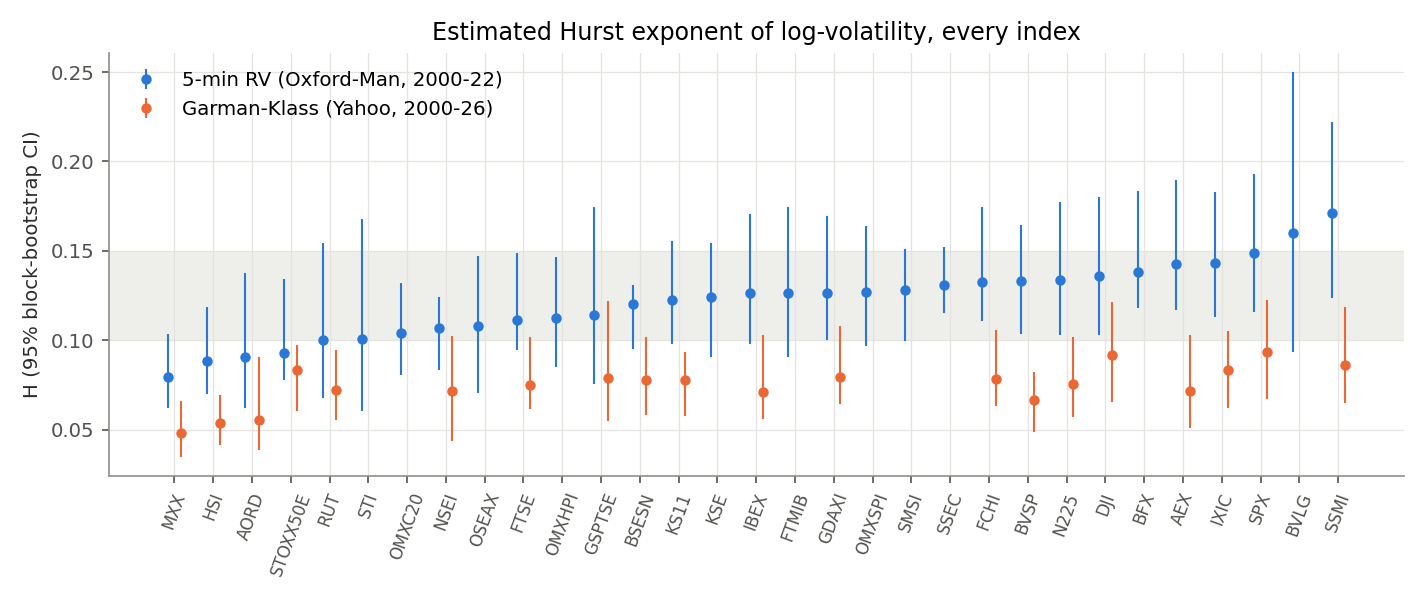
\includegraphics[width=0.92\textwidth]{../figures/h_by_index.png}
\caption{$H$ with 95\% block-bootstrap intervals for every index; the shaded band is $[0.10,0.15]$.}
\label{fig:h}
\end{figure}

\subsection{Gaussianity of increments}
GJR report that $\log\sigma_{t+\Delta}-\log\sigma_t$ is close to Gaussian at all lags. The histograms for
SPX (notebook, Fig.~\texttt{gauss\_spx.png}) are bell-shaped and close to the normal density at
$\Delta=1,5,25,125$. Table~\ref{tab:gauss} gives the median skewness and excess kurtosis over indices:
the skew is small and positive at every lag, but the RV increments have fatter tails than a Gaussian
(excess kurtosis about 2 at one day, 0.8 at 125 days). The Gaussian description is therefore a good
first approximation of the body, not of the tails. For GK the increments look \emph{more} Gaussian, which
is what one expects when a larger, roughly Gaussian measurement error is added.

\begin{table}[h]
\centering\footnotesize
\begin{minipage}{0.42\textwidth}\centering
\begin{tabular}{lrrrr}
\toprule
 & \multicolumn{2}{c}{RV (31)} & \multicolumn{2}{c}{GK (20)}\\
Lag $\Delta$ & skew & exc. kurt. & skew & exc. kurt.\\
\midrule
1 & 0.15 & 2.08 & 0.08 & 0.15\\
5 & 0.19 & 1.70 & 0.08 & 0.38\\
25 & 0.34 & 1.69 & 0.18 & 0.62\\
125 & 0.25 & 0.78 & 0.14 & 0.44\\
\bottomrule
\end{tabular}
\captionof{table}{Median skewness and excess kurtosis of log-vol increments.}\label{tab:gauss}
\end{minipage}\hfill
\begin{minipage}{0.55\textwidth}\centering
\begin{tabular}{rrrr}
\toprule
$H$ true & spot & integrated & integrated + noise\\
\midrule
0.05 & 0.048 & 0.159 & 0.081\\
0.10 & 0.096 & 0.195 & 0.131\\
0.15 & 0.144 & 0.231 & 0.176\\
0.20 & 0.194 & 0.269 & 0.219\\
0.30 & 0.295 & 0.350 & 0.309\\
0.50 & 0.500 & 0.529 & 0.499\\
\bottomrule
\end{tabular}
\captionof{table}{Smoothing bias: mean $\hat H$ over 3 simulated RFSV paths ($\nu=0.3$, 5000 days, 50 steps/day).}\label{tab:sim}
\end{minipage}
\end{table}

\subsection{Smoothing bias}
RV estimates the \emph{integrated} variance $\int_{t-1}^t\sigma_s^2ds$, not spot variance. We simulate
$\log\sigma_t=\nu W^H_t$ exactly (Davies--Harte) on a 50-step intraday grid and estimate $H$ from (i) the spot
log-vol at day ends, (ii) the log of daily integrated variance, (iii) (ii) plus i.i.d.\ noise of s.d.\ 0.25
on log variance. Table~\ref{tab:sim}: the estimator is accurate on spot volatility, daily averaging
biases $\hat H$ \emph{upwards} (0.10 becomes about 0.20 with these parameters), and measurement noise
pulls it back down. The bias is largest for small $H$, so if anything the true $H$ of spot volatility is
smaller than the RV estimates, which strengthens the roughness conclusion. The same mechanism explains
why the noisier GK proxy gives lower $\hat H$ than RV: the two biases act in opposite directions and their
balance depends on the proxy, so $H$ from a daily proxy is not a pure property of the underlying
volatility.

\section{Forecasting method}
\subsection{The RFSV predictor}
Let $X_t=\log\sigma_t$ and assume $X_t=X_0+\nu W^H_t$ with $W^H$ a fBm (the stationary RFSV model adds a
very slow mean reversion that is negligible at horizons of days). For the Mandelbrot--Van Ness fBm
$W^H_t=\frac{1}{C_H}\int_{-\infty}^t\big[(t-s)^{H-1/2}-(-s)_+^{H-1/2}\big]dW_s$, the filtration of $W^H$
equals that of $W$. Splitting $W^H_{t+\Delta}$ into the part driven by $dW_s$, $s\le t$ (known at $t$) and
the part driven by $dW_s$, $s\in(t,t+\Delta]$ (independent of $\mathcal F_t$, mean zero) gives, with $\mathbb E_t=\mathbb E[\,\cdot\,|\mathcal F_t]$ and $a_0=C_H^{-1}\int_{-\infty}^0(-s)^{H-1/2}dW_s$,
\begin{align}
\mathbb E_t[W^H_{t+\Delta}]&=C_H^{-1}{\textstyle\int_{-\infty}^t}(t+\Delta-s)^{H-1/2}dW_s-a_0,\\
\operatorname{Var}_t[W^H_{t+\Delta}]&=\frac{1}{C_H^2}\int_0^\Delta u^{2H-1}du=c\,\Delta^{2H}.
\end{align}
Re-expressing the first integral in terms of the observed past of $W^H$ instead of $W$ (an inversion of
the fractional integral; Nuzman \& Poor, 2000) yields the formula used by GJR:
\begin{equation}\label{eq:rfsv}
\mathbb E[\log v_{t+\Delta}\,|\,\mathcal F_t]=\frac{\cos(H\pi)}{\pi}\,\Delta^{H+1/2}
\int_{-\infty}^t\frac{\log v_s}{(t-s+\Delta)(t-s)^{H+1/2}}\,ds .
\end{equation}
The kernel integrates to one, so the forecast is a weighted average of past log variances with weights
that decay like a power law: recent days dominate, but the whole past matters. With the normalisation
$\operatorname{Var}(W^H_\Delta)=\Delta^{2H}$ one finds
$c=\frac{1}{2H C_H^2}=\frac{\Gamma(3/2-H)}{\Gamma(H+1/2)\Gamma(2-2H)}$ ($c=1$ at $H=1/2$; $c\approx0.64$ at $H=0.1$).
Because $\log v=2X$ is conditionally Gaussian with variance $4c\nu^2\Delta^{2H}$, the variance forecast is
\begin{equation}\label{eq:var}
\mathbb E[v_{t+\Delta}\,|\,\mathcal F_t]=\exp\Big(\mathbb E[\log v_{t+\Delta}|\mathcal F_t]+2c\,\nu^2\Delta^{2H}\Big).
\end{equation}
\emph{Implementation.} The integral is truncated at $L=500$ days. Cell $k$ (lag $u\in[k,k+1)$) gets weight
$w_k\propto\big[(k+1)^{1/2-H}-k^{1/2-H}\big]/\big[(1/2-H)(k+1/2+\Delta)\big]$, i.e.\ the singular factor
$u^{-H-1/2}$ is integrated exactly; weights are normalised to sum to one. $H$ and $\nu$ come from the $q=2$
regression on the past only and are re-estimated every 20 days.

\subsection{Benchmarks and protocol}
\textbf{RW}: $\widehat{\log v}_{t+h}=\log v_t$. \textbf{HAR} (Corsi, 2009) on log variance, direct $h$-step:
$\log v_{t+h}=\beta_0+\beta_d\log v_t+\beta_w\overline{\log v}_{t-4:t}+\beta_m\overline{\log v}_{t-21:t}+\varepsilon$,
re-fitted every day by OLS on all pairs whose target is already observed ($s+h\le t$); the variance
forecast is $\exp(\hat f+\hat s^2/2)$. \textbf{GARCH(1,1)} (Gaussian QMLE, zero mean) on daily returns
(open-to-close for RV, close-to-close for GK), re-fitted every 20 days; because return variance and RV
differ in level, its log and level forecasts are calibrated by the in-sample mean of $\log v_s-\log\sigma^2_s$
and of $v_s/\sigma^2_s$ (past data only).
\textbf{Split.} The first 1000 days of each index are a burn-in. \emph{Validation}: forecasts whose target date
is $\le$ 31-12-2014 (from December 2003). \emph{Test}: origins from 1-1-2015 to the end of each sample
(25-02-2022 for RV, October 2026 for GK). The target is the point value $\log v_{t+h}$, $h\in\{1,5,20\}$ as in GJR.
\textbf{Losses}: MSE of the log-variance forecast (identical ratios for log-vol) and
QLIKE $=v/\hat v-\log(v/\hat v)-1$. Every model is scored on the same days.
\textbf{Tests}: Diebold--Mariano with a Bartlett HAC variance, lag $\max(h,\lfloor4(T/100)^{2/9}\rfloor)$.
We report pairwise DM tests per index; a Model Confidence Set was not run, for cost and simplicity.
\textbf{No look-ahead.} Every model receives only data up to the origin; an automated check perturbs every
observation after a cut-off day and confirms that no forecast made at or before that day changes (it passes for
all models and horizons).

\section{Results}
Table~\ref{tab:test} gives, for the test period, the geometric mean over indices of each model's loss
divided by HAR's loss (below 1 = better than HAR); Table~\ref{tab:dm} counts significant DM wins and losses.

\begin{table}[h]
\centering\scriptsize\setlength{\tabcolsep}{3.6pt}
\resizebox{\textwidth}{!}{\begin{tabular}{lrrrrrr@{\hskip 14pt}rrrrrr}
\toprule
 & \multicolumn{6}{c}{Oxford-Man RV (31 indices)} & \multicolumn{6}{c}{Garman--Klass (20 indices)}\\
 & \multicolumn{3}{c}{MSE / HAR} & \multicolumn{3}{c}{QLIKE / HAR} & \multicolumn{3}{c}{MSE / HAR} & \multicolumn{3}{c}{QLIKE / HAR}\\
Model & 1 & 5 & 20 & 1 & 5 & 20 & 1 & 5 & 20 & 1 & 5 & 20\\
\midrule
RW & 1.338 & 1.391 & 1.444 & 1.458 & 1.534 & 1.907 & 1.499 & 1.564 & 1.600 & 2.146 & 2.348 & 2.649\\
GARCH & 1.333 & 1.179 & 1.152 & 1.302 & 1.147 & 0.983 & 1.154 & 1.106 & 1.118 & 1.095 & 1.043 & 0.950\\
HAR & 1.000 & 1.000 & 1.000 & 1.000 & 1.000 & 1.000 & 1.000 & 1.000 & 1.000 & 1.000 & 1.000 & 1.000\\
RFSV & 1.024 & 1.001 & 0.996 & 1.009 & 1.002 & 1.079 & 1.059 & 1.015 & 0.996 & 1.060 & 1.019 & 1.065\\
\midrule
RFSV-roll250 & 1.031 & 1.014 & \textbf{1.008} & 1.015 & 1.024 & 1.144 & 1.062 & 1.021 & 1.001 & 1.089 & 1.029 & 1.101\\
RFSV-roll500 & 1.032 & 1.012 & 1.006 & 1.016 & 1.015 & 1.110 & 1.061 & 1.019 & 1.000 & 1.073 & 1.027 & 1.081\\
RFSV-roll1000 & 1.025 & 1.005 & 0.999 & 1.011 & 1.009 & 1.097 & 1.062 & 1.018 & 0.999 & 1.066 & 1.024 & 1.078\\
\midrule
HAR-L & 0.954 & 0.987 & 0.992 & 0.957 & 0.990 & 0.999 & 0.944 & 0.979 & 0.994 & 0.929 & 0.968 & 0.993\\
HAR-RFSV & 0.990 & 0.989 & 0.981 & 0.993 & 1.009 & 1.036 & 0.989 & 0.988 & 0.979 & 0.993 & 1.010 & 1.023\\
HAR-L-RFSV & \textbf{0.941} & 0.973 & 0.975 & 0.946 & 0.998 & 1.036 & \textbf{0.933} & \textbf{0.965} & 0.974 & 0.919 & 0.973 & 1.006\\
\midrule
COMB(RFSV,HAR) & 0.996 & 0.993 & 0.991 & 0.992 & 0.994 & 1.057 & 0.995 & 0.997 & 0.990 & 0.993 & 0.998 & 1.038\\
COMB(RFSV,HAR-L) & 0.952 & \textbf{0.982} & 0.987 & 0.952 & 0.985 & 1.051 & 0.941 & 0.978 & \textbf{0.986} & 0.926 & 0.970 & 1.028\\
\bottomrule
\end{tabular}}
\caption{Test period (2015--), loss relative to HAR, geometric mean over indices. Bold: the model chosen
on the validation period for that data set and horizon. Lines below the first block are the improvement candidates.}
\label{tab:test}
\end{table}

\textbf{RFSV against HAR.} On RV data the RFSV predictor is 2.4\% worse than HAR at one day (better on only 5 of 31
indices; significantly worse on 17), level at five days (1.001) and 0.4\% better at twenty days (better on 15 of 31,
significant on none). On GK data it is worse at 1 and 5 days on every index and level at 20 days. In QLIKE, RFSV is
clearly worse than HAR at 20 days (1.079 on RV), and the best QLIKE at 20 days is the calibrated GARCH
(0.983 RV, 0.950 GK), whose level calibration copes best with the 2020 volatility spike. Both RFSV and HAR beat the
random walk and GARCH in log-MSE everywhere. For the S\&P 500 alone RFSV does beat HAR at one day (ratio 0.967),
closer to GJR's SPX result, but this does not generalise across indices.

\begin{table}[h]
\centering\footnotesize
\begin{tabular}{llrcccc}
\toprule
Data & Comparison (A vs B) & $h$ & \multicolumn{2}{c}{log-MSE: A better / worse} & \multicolumn{2}{c}{QLIKE: A better / worse}\\
\midrule
RV & RFSV vs HAR & 1 & 2 & 17 & 2 & 6\\
RV & RFSV vs HAR & 5 & 0 & 4 & 1 & 0\\
RV & RFSV vs HAR & 20 & 0 & 0 & 1 & 0\\
RV & HAR-L-RFSV vs HAR & 1 & 29 & 0 & 22 & 0\\
RV & HAR-L-RFSV vs RFSV & 1 & 30 & 0 & 20 & 0\\
RV & COMB(RFSV,HAR-L) vs HAR & 5 & 21 & 0 & 10 & 0\\
RV & COMB(RFSV,HAR-L) vs RFSV & 5 & 19 & 0 & 9 & 0\\
RV & RFSV-roll250 vs HAR & 20 & 0 & 1 & 0 & 4\\
RV & RFSV-roll250 vs RFSV & 20 & 0 & 8 & 0 & 14\\
\midrule
GK & RFSV vs HAR & 1 & 0 & 18 & 0 & 8\\
GK & RFSV vs HAR & 5 & 0 & 4 & 0 & 1\\
GK & RFSV vs HAR & 20 & 1 & 1 & 0 & 0\\
GK & HAR-L-RFSV vs HAR & 1 & 20 & 0 & 20 & 0\\
GK & HAR-L-RFSV vs RFSV & 1 & 20 & 0 & 19 & 0\\
GK & HAR-L-RFSV vs HAR & 5 & 18 & 0 & 6 & 0\\
GK & HAR-L-RFSV vs RFSV & 5 & 18 & 0 & 12 & 0\\
GK & COMB(RFSV,HAR-L) vs HAR & 20 & 6 & 0 & 0 & 0\\
GK & COMB(RFSV,HAR-L) vs RFSV & 20 & 4 & 0 & 2 & 0\\
\bottomrule
\end{tabular}
\caption{Diebold--Mariano tests on the test period: number of indices (of 31 RV, 20 GK) where A is
significantly better / worse than B at 5\%.}
\label{tab:dm}
\end{table}

\section{Improvements}
Candidates: (i) RFSV with $H,\nu$ from a rolling window of 250, 500 or 1000 days (adaptive $H$);
(ii) HAR-L, HAR with the leverage terms $r_t^-$, $\overline{r^-}_{t-4:t}$, $\overline{r^-}_{t-21:t}$ (Corsi \& Ren\`o, 2012);
(iii) HAR-RFSV, HAR with the real-time RFSV forecast as a fifth regressor; (iv) HAR-L-RFSV, both;
(v) COMB, $w\,\text{RFSV}+(1-w)\,\text{HAR(-L)}$ with $w\in[0,1]$ re-estimated every day by least squares on past
realised forecast errors. One model per data set and horizon is chosen by the lowest validation log-MSE ratio to HAR
(validation table in the notebook), then evaluated once on the test period.

Chosen on validation (RV): HAR-L-RFSV at $h=1$, COMB(RFSV, HAR-L) at $h=5$, RFSV-roll250 at $h=20$;
(GK): HAR-L-RFSV at $h=1,5$, COMB(RFSV, HAR-L) at $h=20$. On the test period:

\begin{center}\footnotesize
\begin{tabular}{lrrrrrr}
\toprule
& \multicolumn{3}{c}{RV, log-MSE / HAR} & \multicolumn{3}{c}{GK, log-MSE / HAR}\\
& $h=1$ & $h=5$ & $h=20$ & $h=1$ & $h=5$ & $h=20$\\
\midrule
RFSV (paper) & 1.024 & 1.001 & 0.996 & 1.059 & 1.015 & 0.996\\
Selected model & \textbf{0.941} & \textbf{0.982} & 1.008 & \textbf{0.933} & \textbf{0.965} & \textbf{0.986}\\
\quad indices where it beats HAR & 31/31 & 31/31 & 8/31 & 20/20 & 20/20 & 19/20\\
\quad indices where it beats RFSV & 31/31 & 30/31 & 1/31 & 20/20 & 20/20 & 20/20\\
\bottomrule
\end{tabular}
\end{center}

The improvement beats both benchmarks at 1 and 5 days on both data sets, significantly on most indices
(Table~\ref{tab:dm}), and at 20 days on GK (significant against HAR on 6 of 20 indices). At 20 days on RV it
fails: the rolling-$H$ RFSV that won the validation period is worse than HAR and than the expanding-window
RFSV on the test period. Most of the short-horizon gain comes from the leverage term: HAR-L alone gives
0.954 / 0.987 / 0.992 (RV), and adding the RFSV forecast lowers this to 0.941 / 0.973 / 0.975. (HAR-L-RFSV was also
the best test model at 20 days, but it was not the validation choice, so we do not claim it.) In QLIKE the
selected models beat HAR at 1 and 5 days (0.946 and 0.985 on RV) but not at 20 days.

\begin{figure}[h]
\centering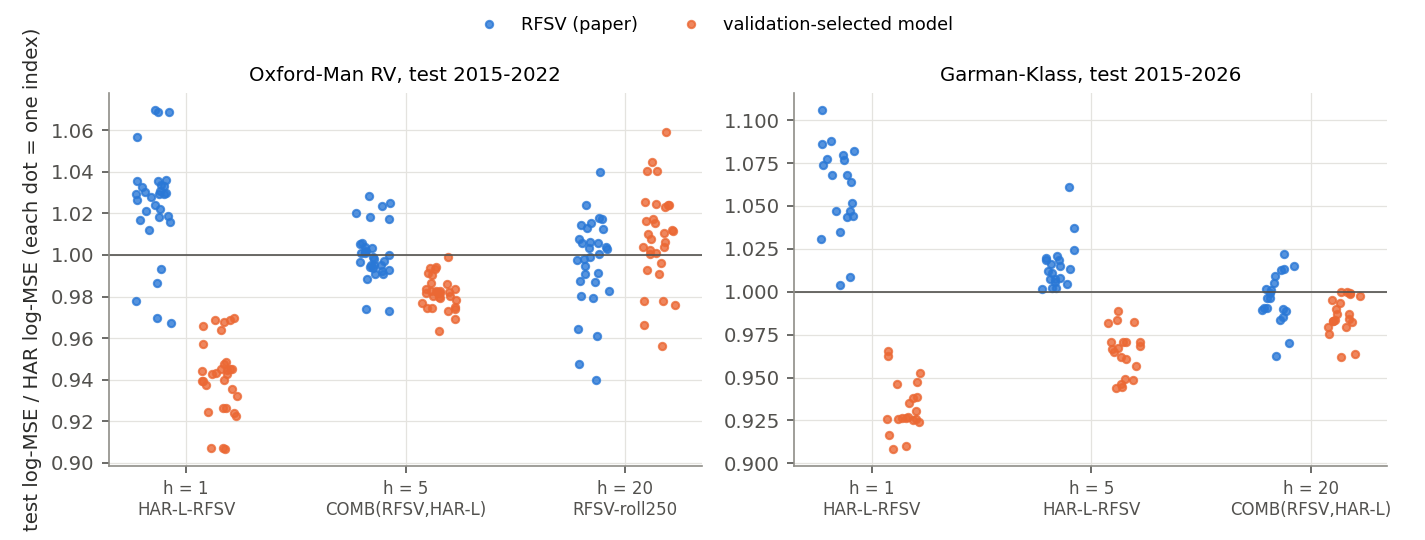
\includegraphics[width=0.92\textwidth]{../figures/test_ratios.png}
\caption{Test-period log-MSE relative to HAR, one dot per index: RFSV (blue) and the validation-selected model (orange).}
\label{fig:test}
\end{figure}

\section{Limitations}
\begin{itemize}\itemsep1pt
\item The RV sample ends in February 2022, when the Oxford-Man library stopped; post-2022 results rely on the
noisier range-based proxy, whose $H$ is not comparable in level with RV-based $H$.
\item $H$ estimated from daily proxies is biased upwards by daily integration and downwards by noise
(Table~\ref{tab:sim}); we did not correct for either.
\item The target is point RV $h$ days ahead (as in GJR), not the average over the next $h$ days; HAR is usually
specified for the latter, and rankings could differ.
\item Variance (QLIKE) forecasts depend heavily on the level correction. The paper's correction
(\ref{eq:var}) uses $\nu$ estimated from noisy RV; all models under-predict the mean level in the test period
(mean $v/\hat v$ above 1, driven by spikes such as March 2020).
\item Indices are not independent (cross-market correlation), so the DM counts are not independent tests.
No Model Confidence Set and no multiple-testing correction across the 8 candidates (the validation step is the
only guard against selection bias).
\item Yahoo index OHLC is not an audited source; we cleaned obvious errors only.
\end{itemize}

\section*{References}
\small
\begin{itemize}\itemsep0pt
\item[] Corsi, F. (2009). A simple approximate long-memory model of realized volatility. \emph{J. Financial Econometrics} 7(2), 174--196.
\item[] Corsi, F. \& Ren\`o, R. (2012). Discrete-time volatility forecasting with persistent leverage effect and the link with continuous-time volatility modeling. \emph{J. Business \& Economic Statistics} 30(3), 368--380.
\item[] Diebold, F.X. \& Mariano, R.S. (1995). Comparing predictive accuracy. \emph{J. Business \& Economic Statistics} 13(3), 253--263.
\item[] Garman, M.B. \& Klass, M.J. (1980). On the estimation of security price volatilities from historical data. \emph{J. Business} 53(1), 67--78.
\item[] Gatheral, J., Jaisson, T. \& Rosenbaum, M. (2018). Volatility is rough. \emph{Quantitative Finance} 18(6), 933--949. arXiv:1410.3394.
\item[] Heber, G., Lunde, A., Shephard, N. \& Sheppard, K. (2009). Oxford-Man Institute's realized library, version 0.3.
\item[] Hansen, P.R., Lunde, A. \& Nason, J.M. (2011). The model confidence set. \emph{Econometrica} 79(2), 453--497.
\item[] Mandelbrot, B. \& Van Ness, J. (1968). Fractional Brownian motions, fractional noises and applications. \emph{SIAM Review} 10(4), 422--437.
\item[] Nuzman, C.J. \& Poor, H.V. (2000). Linear estimation of self-similar processes via Lamperti's transformation. \emph{J. Applied Probability} 37(2), 429--452.
\item[] Parkinson, M. (1980). The extreme value method for estimating the variance of the rate of return. \emph{J. Business} 53(1), 61--65.
\item[] Patton, A.J. (2011). Volatility forecast comparison using imperfect volatility proxies. \emph{J. Econometrics} 160(1), 246--256.
\end{itemize}
\end{document}
